% Day 3 - Moored floating box: hands-on background (FoamWaveTank training)
% Build:  pdflatex Day3_MooredBox_HandsOn.tex  (run twice)
\documentclass[aspectratio=169,10pt]{beamer}

\usepackage[T1]{fontenc}
\usepackage{lmodern}
\usepackage{amsmath}
\usepackage{booktabs}
\usepackage{tabularx}
\usepackage{array}
\newcolumntype{L}{>{\raggedright\arraybackslash}X}
\newcolumntype{P}[1]{>{\raggedright\arraybackslash}p{#1}}
\usepackage{listings}
\usepackage{tikz}
\usepackage{pgfplots}
\pgfplotsset{compat=1.17}
\usetikzlibrary{arrows.meta,positioning,calc,shapes.geometric,decorations.pathmorphing}

% ---------------------------------------------------------------- colours
\definecolor{deep}{HTML}{0B3C49}
\definecolor{sea}{HTML}{1A7F8E}
\definecolor{foam}{HTML}{EAF4F4}
\definecolor{sand}{HTML}{F2A541}
\definecolor{coral}{HTML}{C8414F}
\definecolor{ink}{HTML}{1F2A30}
\definecolor{mute}{HTML}{5C6B73}
\definecolor{codebg}{HTML}{F3F6F7}

% ---------------------------------------------------------------- beamer look
\usetheme{default}
\setbeamertemplate{navigation symbols}{}
\setbeamercolor{normal text}{fg=ink}
\setbeamercolor{frametitle}{fg=deep}
\setbeamercolor{structure}{fg=sea}
\setbeamercolor{alerted text}{fg=coral}
\setbeamerfont{frametitle}{size=\Large,series=\bfseries}
\setbeamertemplate{itemize items}{\color{sea}\raisebox{0.15ex}{\tiny$\blacksquare$}}
\setbeamertemplate{itemize subitem}{\color{mute}--}
\setbeamertemplate{enumerate items}[default]
\setbeamertemplate{frametitle}{\vspace*{0.3em}\insertframetitle\par\vspace*{-0.2em}}
\setbeamertemplate{footline}{%
  \hbox{\hspace*{1em}\color{mute}\tiny FoamWaveTank training \,$\cdot$\, Day 3: Moored box
  \hfill\insertframenumber\hspace*{1em}}\vspace*{0.6em}}

\newcommand{\sectionframe}[2]{%
  {\setbeamercolor{background canvas}{bg=deep}
   \setbeamertemplate{footline}{}
   \begin{frame}[plain]
     \vfill
     {\color{sand}\large\bfseries #1}\par\vspace{0.4em}
     {\color{white}\huge\bfseries #2}
     \vfill
   \end{frame}}}

\newcommand{\file}[1]{{\leavevmode\ttfamily\color{deep}#1}}
\newcommand{\key}[1]{{\leavevmode\ttfamily\color{sea}#1}}

% ---------------------------------------------------------------- listings
\lstdefinelanguage{foam}{
  morecomment=[l]{//}, morecomment=[s]{/*}{*/}, morecomment=[l]{\#},
  morestring=[b]",
  morekeywords={waveType,height,period,depth,direction,phi,Tsoft,
    relaxationZone,relaxationScheme,relaxationShape,beachType,relaxType,startX,endX,orientation,
    spectrum,Hs,Tp,gamma,N,phaseMethod,seedForRandomPhase,frequencyAxis,etaMax,focusTime,focusPoint,
    seaLevel,relaxationNames,initializationName,externalForcing,Grid2Grid,Grid2GridCoeffs,
    Grid2GridInputFileName,referencePosition,referenceTheta,referenceTime,
    type,fileType,filePath,interpolationOrder,zMeshType,zMin,zMax,nZMin,nZMax,zMinRatio,zMaxRatio,
    pointDistribution,xValues,yValues,zValues,add,axis,writeControl,writeInterval,
    inletCoeffs,outletCoeffs,U,discretisation,lowerFrequencyCutoff,upperFrequencyCutoff,writeSpectrum}
}
\lstset{
  basicstyle=\ttfamily\scriptsize\color{ink},
  keywordstyle=\color{sea}\bfseries,
  commentstyle=\color{mute}\itshape,
  stringstyle=\color{coral},
  backgroundcolor=\color{codebg},
  frame=none, framesep=0pt, xleftmargin=4pt, xrightmargin=4pt,
  aboveskip=2pt, belowskip=2pt,
  columns=fullflexible, keepspaces=true, showstringspaces=false,
  breaklines=false, tabsize=4, upquote=true
}
\lstdefinestyle{sh}{language=bash, morekeywords={runApplication,python3,cd,cp},
  keywordstyle=\color{sea}\bfseries}

\tikzset{
  box/.style={draw=sea, fill=foam, rounded corners=3pt, thick, align=center,
              font=\scriptsize, inner sep=4pt},
  dbox/.style={draw=deep, fill=deep, text=white, rounded corners=3pt, thick, align=center,
               font=\scriptsize\bfseries, inner sep=4pt},
  arr/.style={-{Stealth[length=2.5mm]}, thick, color=deep},
}

\lstdefinelanguage{foamb}[]{foam}{morekeywords={dynamicFvMesh,motionSolverLibs,motionSolver,
  sixDoFRigidBodyMotionCoeffs,solvers,floaterMeshMotionSolverCoeffs,patches,innerDistance,
  outerDistance,linDirs,rotDirs,MaddUpdateFreq,addedMassModel,restraints,mass,centreOfMass,
  momentOfInertia,accelerationRelaxation,report,rho,solver,constraints,centreOfRotation,orientation,
  initialCentreOfRotation,initialOrientation,initialCentreOfMass,waveModel,nPaddle,waveHeight,
  waveAngle,rampTime,activeAbsorption,wavePeriod,alpha,sixDoFRigidBodyMotionRestraint,
  floaterMotionRestraint,couplingMode,inputFile,vtkPrefix,writeMooringVTK,vtkStartTime,outerCorrector,
  nxCells,nxBox,nz_L1A5,nz_L2A4,nz_Box,box,moorDynR2_body}}

\title{Day 3: Moored floating box}
\date{}

\begin{document}

% ======================================================================
{\setbeamercolor{background canvas}{bg=deep}
 \setbeamertemplate{footline}{}
\begin{frame}[plain]
  \vfill
  {\color{sand}\large\bfseries FoamWaveTank training}\par\vspace{0.5em}
  {\color{white}\fontsize{30}{34}\selectfont\bfseries Day 3: Moored floating box}\par\vspace{0.8em}
  {\color{foam}\normalsize Hands-on background: mooring dynamics with MoorDyn, coupling to the
   body solver,\\ mesh, waves, set-up, output, mooring in ParaView and HOS waves}
  \vfill
  
\begin{tikzpicture}
    \draw[sand, very thick, domain=0:14, samples=200] plot (\x, {0.2*sin(deg(2*pi*\x/4))});
    \fill[foam] (6.6,-0.25) rectangle (7.4,0.4);
    \draw[foam, thick] (6.6,-0.25) .. controls (5.6,-1.2) and (4.8,-1.3) .. (4.0,-1.35);
    \draw[foam, thick] (7.4,-0.25) .. controls (8.4,-1.2) and (9.2,-1.3) .. (10.0,-1.35);
    \fill[foam] (4.0,-1.35) circle (2pt); \fill[foam] (10.0,-1.35) circle (2pt);
  \end{tikzpicture}
  \vfill
\end{frame}}

% ======================================================================
\begin{frame}{The day: a box on four mooring lines}
  \centering
  
\begin{tikzpicture}[node distance=6mm]
    \node[dbox, minimum width=4.2cm, minimum height=1cm] (a) {\texttt{waveIsoFoam/mooredBox}\\sixDoF + MoorDyn};
    \node[dbox, minimum width=4.2cm, minimum height=1cm, right=of a, fill=sea, draw=sea] (b) {\texttt{FloatStepper/mooredBox}\\FloatStepper + MoorDyn};
    \node[dbox, minimum width=4.2cm, minimum height=1cm, right=of b, fill=coral, draw=coral] (c) {\texttt{HOS\_FloatStepper/}\\the same in HOS waves};
  \end{tikzpicture}

  \vspace{4mm}
  \begin{columns}[T]
    \column{0.42\textwidth}\small
    \begin{itemize}
      \item Same mesh, box, mooring input and wave in the first two
      \item Wave: StokesII, $H$ = 0.1195 m, $T$ = 1.993 s, depth 0.5 m
      \item Tank $x$ = $-2.5$ \dots 2.5 m, box at $x$ = 0
      \item 10 gauges $x$ = $-2$ \dots 2 m, line tensions in \file{Mooring/}
      \item \texttt{endTime} 23 s: the full experiment window
    \end{itemize}
    \column{0.55\textwidth}\footnotesize
    \renewcommand{\arraystretch}{1.15}
    \begin{tabular}{@{}lrrr@{}}
      \toprule
      Mesh & Cells & waveIsoFoam & FloatStepper \\
      \midrule
      medium (default) & 3760 & 12 min & 20 min \\
      coarse & 1088 & 6 min & 8 min \\
      \bottomrule
    \end{tabular}

    \vspace{2mm}
    \scriptsize Serial, one DTU HPC core. \texttt{MESH=coarse ./Allrun}. The coarse mesh is a quick look only: its pitch
    amplitude is about 60\,\% of the medium-mesh one.
  \end{columns}
\end{frame}

% ======================================================================
\sectionframe{Part 1}{The moored box and MoorDyn}

% ----------------------------------------------------------------------
\begin{frame}{The experiment: Wu et al.\ (2019), box BOX3}
  \centering
  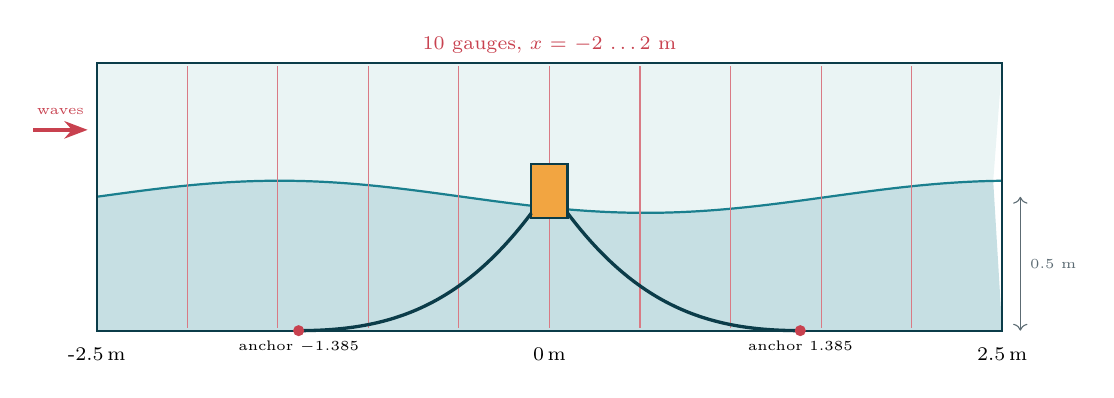
\begin{tikzpicture}[x=2.3cm, y=3.4cm]
    \fill[sea!25] (-2.5,-0.5) -- (-2.5,0) \foreach \x in {-2.5,-2.45,...,2.5} { -- (\x,{0.06*sin(deg(2*pi*(\x+2.5)/4.04))}) } -- (2.5,-0.5) -- cycle;
    \fill[foam] (-2.5,0) \foreach \x in {-2.5,-2.45,...,2.5} { -- (\x,{0.06*sin(deg(2*pi*(\x+2.5)/4.04))}) } -- (2.5,0.5) -- (-2.5,0.5) -- cycle;
    \draw[sea, thick, domain=-2.5:2.5, samples=200] plot (\x,{0.06*sin(deg(2*pi*(\x+2.5)/4.04))});
    \draw[deep, thick] (-2.5,-0.5) rectangle (2.5,0.5);
    \foreach \x in {-2,-1.5,...,2} \draw[coral!70, thin] (\x,-0.49) -- (\x,0.49);
    \fill[sand, draw=deep, thick] (-0.1,-0.0786) rectangle (0.1,0.1214);
    \draw[deep, very thick] (-0.1,-0.061) .. controls (-0.5,-0.42) and (-0.9,-0.5) .. (-1.385,-0.5);
    \draw[deep, very thick] (0.1,-0.061) .. controls (0.5,-0.42) and (0.9,-0.5) .. (1.385,-0.5);
    \fill[coral] (-1.385,-0.5) circle (2pt); \fill[coral] (1.385,-0.5) circle (2pt);
    \node[font=\tiny, below] at (-1.385,-0.5) {anchor $-1.385$};
    \node[font=\tiny, below] at (1.385,-0.5) {anchor 1.385};
    \foreach \x in {-2.5,0,2.5} \node[font=\scriptsize, below] at (\x,-0.53) {\x\,m};
    \node[font=\scriptsize, coral, above] at (0,0.5) {10 gauges, $x$ = $-2$ \dots 2 m};
    \draw[coral, very thick, -{Stealth}] (-2.85,0.25) -- (-2.55,0.25);
    \node[font=\tiny, coral] at (-2.7,0.32) {waves};
    \draw[<->, mute] (2.6,-0.5) -- node[right, font=\tiny] {0.5 m} (2.6,0);
  \end{tikzpicture}

  \vspace{1mm}
  \begin{columns}[T]
    \column{0.32\textwidth}\small
    \textbf{Box}
    \begin{itemize}
      \item 0.2 m $\times$ 0.2 m, 0.2 m wide (the 2D slice is the box width)
      \item draft 0.0786 m, 3.148 kg
      \item CoG $z$ = $-0.0126$ m
    \end{itemize}
    \column{0.32\textwidth}\small
    \textbf{Wave}: StokesII
    \begin{itemize}
      \item $H$ = 0.1195 m, $T$ = 1.993 s
      \item $L$ = 4.04 m, $kh$ = 0.78
      \item $H/L$ = 0.030
    \end{itemize}
    \column{0.32\textwidth}\small
    \textbf{Mooring}
    \begin{itemize}
      \item 4 slack lines, 1.455 m each
      \item seabed anchors, fairleads on the box bottom corners
      \item 3D lines on a 2D CFD box
    \end{itemize}
  \end{columns}
\end{frame}

% ----------------------------------------------------------------------
\begin{frame}{Mooring layout (plan view)}
  \begin{columns}[T]
    \column{0.5\textwidth}
    \centering
    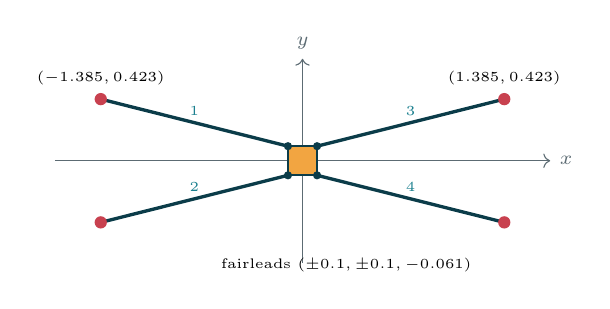
\begin{tikzpicture}[scale=1.85]
      \draw[mute, ->] (-1.7,0) -- (1.7,0) node[right, font=\scriptsize] {$x$};
      \draw[mute, ->] (0,-0.7) -- (0,0.7) node[above, font=\scriptsize] {$y$};
      \fill[sand, draw=deep, thick] (-0.1,-0.1) rectangle (0.1,0.1);
      \foreach \ax/\ay/\bx/\by/\n in {-1.385/0.423/-0.1/0.1/1, -1.385/-0.423/-0.1/-0.1/2, 1.385/0.423/0.1/0.1/3, 1.385/-0.423/0.1/-0.1/4} {
        \draw[deep, very thick] (\ax,\ay) -- (\bx,\by);
        \fill[coral] (\ax,\ay) circle (1.2pt);
        \fill[deep] (\bx,\by) circle (0.8pt);
        \node[font=\tiny, sea] at ($(\ax,\ay)!0.5!(\bx,\by) + (0,0.08)$) {\n};
      }
      \node[font=\tiny, above] at (-1.385,0.45) {$(-1.385, 0.423)$};
      \node[font=\tiny, above] at (1.385,0.45) {$(1.385, 0.423)$};
      \node[font=\tiny, below] at (0.3,-0.6) {fairleads $(\pm0.1, \pm0.1, -0.061)$};
    \end{tikzpicture}

    \small anchors at $z$ = $-0.5$ (bed), fairleads in body coordinates
    \column{0.47\textwidth}\small
    \textbf{Line properties} (\file{Mooring/lines\_v2\_bodyC.txt})

    \vspace{1mm}
    \renewcommand{\arraystretch}{1.12}
    \begin{tabular}{@{}ll@{}}
      \toprule
      diameter & 3.656 mm \\
      mass per length & 0.0607 kg/m \\
      axial stiffness $EA$ & 29 N \\
      unstretched length & 1.455 m \\
      segments per line & 40 \\
      $C_d$ / $C_a$ (normal) & 1.6 / 1.0 \\
      $C_d$ / $C_a$ (axial) & 0.05 / 0 \\
      \bottomrule
    \end{tabular}

    \vspace{2mm}
    $EA$ = 29 N is soft: an elastic (rubber-like) line. The lines are slack: the box moves on
    the line weight and stretch.
  \end{columns}
\end{frame}

% ----------------------------------------------------------------------
\begin{frame}{MoorDyn: a lumped-mass line model}
  \begin{columns}[T]
    \column{0.55\textwidth}\small
    Each line is split into $N$ segments. The mass sits at the nodes, which are joined by
    axial springs and dampers:
    \[
      (m_i + a_i)\,\ddot{\mathbf{r}}_i = \mathbf{T}_{i+\frac12} - \mathbf{T}_{i-\frac12}
      + \mathbf{C} + \mathbf{W}_i + \mathbf{B}_i + \mathbf{D}_i
    \]
    \begin{itemize}
      \item $\mathbf{T}$: tension, $EA\,\varepsilon$ (only in stretch, no compression)
      \item $\mathbf{C}$: internal damping (\texttt{BA/-zeta} = $-1$: critical-damping fraction)
      \item $\mathbf{W}$, $\mathbf{B}$: weight and buoyancy
      \item $\mathbf{D}$, $a_i$: Morison drag and added mass, normal and axial
      \item seabed contact as a stiff spring--damper (\texttt{kBot}, \texttt{cBot})
    \end{itemize}
    Time integration: RK4 with \texttt{dtM} = $10^{-4}$ s, many substeps inside one CFD step.

    \vspace{1mm}
    \scriptsize Hall \& Goupee, Ocean Eng.\ 104 (2015); Chen \& Hall, Appl.\ Ocean Res.\ 124 (2022)
    \column{0.42\textwidth}
    \centering
    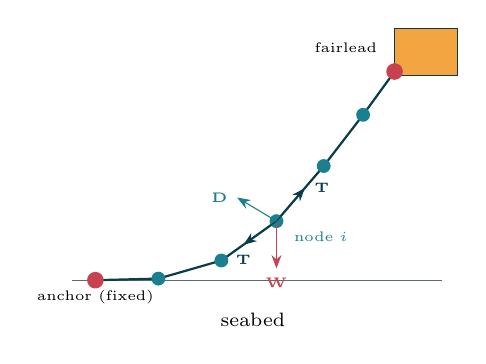
\begin{tikzpicture}[scale=1]
      \draw[mute] (-0.3,0) -- (4.4,0);
      \fill[sand, draw=deep] (3.8,2.6) rectangle (4.6,3.2);
      \coordinate (p0) at (0,0);
      \coordinate (p1) at (0.8,0.02);
      \coordinate (p2) at (1.6,0.25);
      \coordinate (p3) at (2.3,0.75);
      \coordinate (p4) at (2.9,1.45);
      \coordinate (p5) at (3.4,2.1);
      \coordinate (p6) at (3.8,2.65);
      \draw[deep, thick] (p0) -- (p1) -- (p2) -- (p3) -- (p4) -- (p5) -- (p6);
      \foreach \p in {p1,p2,p3,p4,p5} \fill[sea] (\p) circle (2.5pt);
      \fill[coral] (p0) circle (3pt); \fill[coral] (p6) circle (3pt);
      \draw[-{Stealth}, coral] (p3) -- ++(0,-0.6) node[below, font=\tiny] {$\mathbf{W}$};
      \draw[-{Stealth}, deep] (p3) -- ($(p3)!0.6!(p4)$) node[right, font=\tiny] {$\mathbf{T}$};
      \draw[-{Stealth}, deep] (p3) -- ($(p3)!0.6!(p2)$) node[below, font=\tiny] {$\mathbf{T}$};
      \draw[-{Stealth}, sea] (p3) -- ++(-0.5,0.3) node[left, font=\tiny] {$\mathbf{D}$};
      \node[font=\tiny, below] at (p0) {anchor (fixed)};
      \node[font=\tiny, left] at (3.7,2.95) {fairlead};
      \node[font=\tiny, sea, right] at (2.4,0.55) {node $i$};
      \node[font=\scriptsize] at (2,-0.5) {seabed};
    \end{tikzpicture}
  \end{columns}
\end{frame}

% ----------------------------------------------------------------------
\begin{frame}[fragile]{The MoorDyn v2 input file}
  \begin{columns}[T]
    \column{0.6\textwidth}
\begin{lstlisting}[basicstyle=\ttfamily\tiny\color{ink}]
------------------- LINE TYPES -----------------------------------
TypeName Diam     Mass/m  EA   BA/-zeta EI  Cd   Ca   CdAx CaAx
main     0.003656 0.0607  29   -1.0     0   1.6  1.0  0.05 0.0
------------------- BODIES ---------------------------------------
ID Attachment X0 Y0 Z0      r0 p0 y0 Mass  CG* I* Volume CdA* Ca
1  Coupled    0  0  -0.0126 0  0  0  3.148 0   0  0      0    0
------------------- CONNECTION PROPERTIES ------------------------
ID Type   X      Y      Z      Mass Volume CdA Ca
1  Fixed  -1.385  0.423 -0.5   0    0      0   0    # anchors 1-4
...
5  Body1  -0.1    0.1   -0.061 0    0      0   0    # fairleads 5-8
...
------------------- LINES ----------------------------------------
ID LineType AttachA AttachB UnstrLen NumSegs LineOutputs
1  main     1       5       1.455    40      pt
...
------------------- OPTIONS --------------------------------------
1e-4   dtM       - time step of the mooring integration
RK4    tScheme   - time integration scheme
0      WaveKin   - wave kinematics (0 = neglect)
3.0e6  kBot      - bottom stiffness (Pa/m)
3.0e5  cBot      - bottom damping (Pa-s/m)
0.5    WtrDpth   - water depth (m)
------------------- OUTPUTS --------------------------------------
B1PX  B1PY  B1PZ  FAIRTEN1  FAIRTEN3  ANCHTEN1  ANCHTEN3
\end{lstlisting}
    \column{0.37\textwidth}\small
    \begin{itemize}
      \item \textbf{BODIES}: \texttt{Coupled}: the CFD moves this body. Mass and inertia come from
            the CFD, so they are 0 here
      \item \textbf{CONNECTIONS}: \texttt{Fixed} anchors, \texttt{Body1} fairleads (in body coordinates)
      \item \textbf{LINES}: from anchor to fairlead. \texttt{pt}: write node positions and tensions
      \item \textbf{OPTIONS}: \texttt{WaveKin 0}: the lines do not feel the waves, only still water
      \item \textbf{OUTPUTS}: body position, tensions at fairleads and anchors
    \end{itemize}
    \scriptsize \texttt{ICgenDynamic}: before $t$ = 0 MoorDyn lets the lines settle (up to \texttt{TmaxIC} = 5 s).
  \end{columns}
\end{frame}

% ----------------------------------------------------------------------
\begin{frame}{Coupling the body to MoorDyn (\texttt{moorDynR2})}
  \centering
  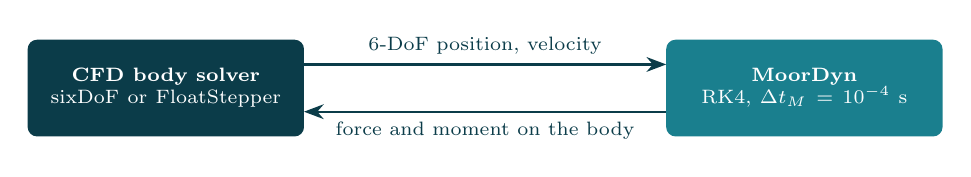
\begin{tikzpicture}[node distance=7mm]
    \node[dbox, text width=3.2cm, minimum height=1.2cm] (c) {CFD body solver\\{\normalfont sixDoF or FloatStepper}};
    \node[dbox, text width=3.2cm, minimum height=1.2cm, right=4.6cm of c, fill=sea, draw=sea] (m) {MoorDyn\\{\normalfont RK4, $\Delta t_M = 10^{-4}$ s}};
    \draw[arr] ([yshift=3mm]c.east) -- node[above, font=\scriptsize] {6-DoF position, velocity} ([yshift=3mm]m.west);
    \draw[arr] ([yshift=-3mm]m.west) -- node[below, font=\scriptsize] {force and moment on the body} ([yshift=-3mm]c.east);
  \end{tikzpicture}

  \vspace{4mm}
  \begin{columns}[T]
    \column{0.48\textwidth}\small
    \begin{itemize}
      \item The mooring is a \textbf{restraint} of the body: an extra force and moment in Newton--Euler
      \item \texttt{couplingMode "BODY"}: OpenFOAM passes the whole body state; MoorDyn places the
            fairleads itself. (\texttt{"POINT"}: OpenFOAM passes each fairlead)
      \item Per CFD step MoorDyn integrates from $t$ to $t+\Delta t$ with $\sim\Delta t/\Delta t_M$ substeps
    \end{itemize}
    \column{0.48\textwidth}\small
    \begin{itemize}
      \item \textbf{Save and restore}: when the CFD repeats a step (outer correctors, the FloatStepper
            test step) MoorDyn restarts from the saved state, so it never runs ahead
      \item \texttt{outerCorrector 1}: which outer corrector writes the VTK output
      \item \texttt{writeMooringVTK}: line shapes for ParaView in \file{Mooring/VTK/}
    \end{itemize}
  \end{columns}

  \vspace{2mm}
  \small Library: \file{src/moorDynSixDoF/moorDynR2} (sixDoF) and FloatStepper's \texttt{moorDynR2}, same physics.
\end{frame}

% ======================================================================
\sectionframe{Part 2}{Case set-up}

% ----------------------------------------------------------------------
\begin{frame}[fragile]{\texttt{waveIsoFoam/mooredBox}: sixDoF with a MoorDyn restraint}
  \begin{columns}[T]
    \column{0.52\textwidth}
\begin{lstlisting}[language=foamb]
dynamicFvMesh     dynamicMotionSolverFvMesh;
motionSolverLibs  (sixDoFRigidBodyMotion);
motionSolver      sixDoFRigidBodyMotion;
sixDoFRigidBodyMotionCoeffs
{
    patches         (box);
    innerDistance   0.075;
    outerDistance   0.4;
    mass            3.148;
    centreOfMass    (0 0 -0.0126);
    momentOfInertia (0.015 0.0167 0.021);
    accelerationRelaxation 0.4;
    solver { type Newmark; }  constraints { ... }
    restraints
    {   moorDynR2_body
        {   sixDoFRigidBodyMotionRestraint moorDynR2;
            couplingMode    "BODY";
            inputFile  "Mooring/lines_v2_bodyC.txt";
            vtkPrefix       "mdv2_body";
            writeMooringVTK true;
            vtkStartTime    0;
            outerCorrector  1;
        }
    }
}
\end{lstlisting}
    \column{0.45\textwidth}\small
    \textbf{Different from Day 2}
    \begin{itemize}
      \item \key{motionSolver sixDoFRigidBodyMotion}: the body is in \file{dynamicMeshDict}, not a
            \key{pointDisplacement} BC
      \item Mesh motion: points within \key{innerDistance} (0.075 m) move rigidly, beyond
            \key{outerDistance} (0.4 m) they stay; smooth blend between
      \item \key{restraints}: here the MoorDyn coupling; also springs, dampers
    \end{itemize}
    \textbf{Same as Day 2}
    \begin{itemize}
      \item \key{accelerationRelaxation 0.4}, Newmark, surge--heave--pitch constraints
      \item box: \key{movingWallVelocity}
    \end{itemize}
    \textbf{Output}: \key{sixDoFRigidBodyState} and \key{forces} function objects in
    \file{controlDict}
  \end{columns}
\end{frame}

% ----------------------------------------------------------------------
\begin{frame}[fragile]{\texttt{FloatStepper/mooredBox}: the same mooring}
  \begin{columns}[T]
    \column{0.5\textwidth}
\begin{lstlisting}[language=foamb]
dynamicFvMesh   dynamicPointDisplacementFvMesh;
solvers
{ box
  { motionSolverLibs ( floaterMotion );
    motionSolver    floaterMeshMotionSolver;
    floaterMeshMotionSolverCoeffs
    {
        patches         (box);
        innerDistance   0.075;
        outerDistance   0.4;
        linDirs         (1 0 1);
        rotDirs         (0 1 0);
        addedMassModel  pisoAddedMass;
        MaddUpdateFreq  4;
        restraints
        { moorDynR2_body
          { floaterMotionRestraint moorDynR2;
            couplingMode  "BODY";
            inputFile "Mooring/lines_v2_bodyC.txt";
            ...      // as sixDoF
} } } } }
\end{lstlisting}
    \column{0.47\textwidth}\small
    \file{0.orig/uniform/floaters}
\begin{lstlisting}[language=foamb]
box
{
    centreOfRotation ( 0 0 -0.0126 );
    orientation  ( 1 0 0 0 1 0 0 0 1 );
    velocity     ( 0 0 0 );
    ...
    mass             3.148;
    centreOfMass     $centreOfRotation;
    momentOfInertia  ( 0.015 0 0 0.0167 0 0.021 );
    initialCentreOfRotation $centreOfRotation;
    ...
}
\end{lstlisting}
    \begin{itemize}
      \item Restraint class: \key{floaterMotionRestraint} instead of
            \key{sixDoFRigidBodyMotionRestraint}
      \item Same MoorDyn file, same \key{innerDistance}/\key{outerDistance}
      \item The box starts at its moored equilibrium. It still settles about 5 mm into the mooring
      \item Output: \file{postProcessing/floaterMotion}
    \end{itemize}
  \end{columns}
\end{frame}

% ----------------------------------------------------------------------
\begin{frame}[fragile]{The mesh: blocks around the box, three resolutions}
  \begin{columns}[T]
    \column{0.47\textwidth}
    \centering
    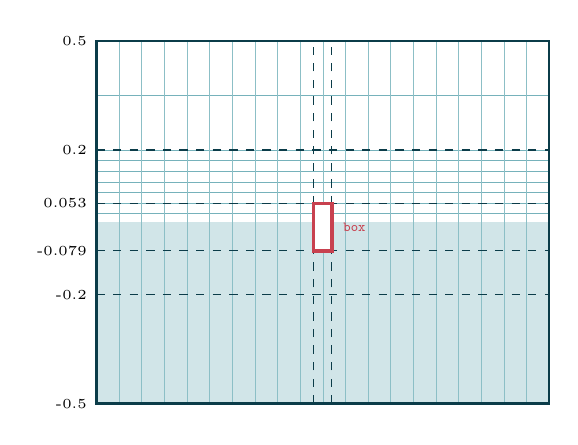
\begin{tikzpicture}[x=1.15cm, y=4.6cm]
      \foreach \za/\zb/\n in {-0.5/-0.2/2, -0.2/-0.0786/5, -0.0786/0.053/5, 0.053/0.2/5, 0.2/0.5/2} {
        \pgfmathsetmacro{\dz}{(\zb-\za)/\n}
        \foreach \i in {1,...,\n} \draw[sea!60, line width=0.2pt] (-2.5,{\za+\i*\dz}) -- (2.5,{\za+\i*\dz});
      }
      \fill[sea!20] (-2.5,-0.5) rectangle (2.5,0);
      \foreach \x in {-2.5,-2.25,...,2.5} \draw[sea!50, line width=0.2pt] (\x,-0.5) -- (\x,0.5);
      \foreach \z in {-0.2,-0.0786,0.053,0.2} \draw[deep, dashed] (-2.5,\z) -- (2.5,\z);
      \draw[deep, dashed] (-0.1,-0.5) -- (-0.1,0.5); \draw[deep, dashed] (0.1,-0.5) -- (0.1,0.5);
      \fill[white] (-0.1,-0.0786) rectangle (0.1,0.053);
      \draw[coral, very thick] (-0.1,-0.0786) rectangle (0.1,0.053);
      \draw[deep, thick] (-2.5,-0.5) rectangle (2.5,0.5);
      \node[font=\tiny, coral, right] at (0.12,-0.012) {\texttt{box}};
      \foreach \z/\l in {-0.5/-0.5,-0.2/-0.2,-0.0786/-0.079,0.053/0.053,0.2/0.2,0.5/0.5} \node[font=\tiny, left] at (-2.5,\z) {\l};
    \end{tikzpicture}

    \scriptsize 14 blocks around a hole: the box patch is part of \file{blockMeshDict}, no
    \texttt{subsetMesh}. Grid lines: every 4th in $x$.
    \column{0.5\textwidth}\small
    \file{system/meshSize.medium} (included by \file{blockMeshDict})
\begin{lstlisting}[language=foamb]
// medium mesh: dx = 0.025 m (L/160)
nxCells     96;    // each side of the box
nxBox       8;     // across the box
nz_L1A5     2;     // bottom / top layer
nz_L2A4     5;     // near the surface
nz_Box      5;     // along the box side
\end{lstlisting}
    \renewcommand{\arraystretch}{1.12}
    \begin{tabular}{@{}lrrl@{}}
      \toprule
      \texttt{MESH=} & $\Delta x$ & cells & use \\
      \midrule
      \texttt{coarse} & 0.05 m & 1088 & quick look \\
      \texttt{medium} & 0.025 m & 3760 & default \\
      \texttt{fine} & 0.0125 m & 15\,040 & waveIsoFoam only \\
      \bottomrule
    \end{tabular}

    \vspace{2mm}
    \texttt{Allrun} copies \file{meshSize.\$MESH} to \file{meshSize}, then \texttt{blockMesh},
    \texttt{setFields} (still water at $z$ = 0) and the solver.
  \end{columns}
\end{frame}

% ----------------------------------------------------------------------
\begin{frame}[fragile]{Waves and numerics}
  \begin{columns}[T]
    \column{0.45\textwidth}
    \small\file{constant/waveProperties}
\begin{lstlisting}[language=foamb]
seaLevel        0;
relaxationNames ();     // no zones
inlet
{
    alpha           alpha.water;
    waveModel       StokesII;
    nPaddle         1;
    waveHeight      0.1195;
    wavePeriod      1.993;
    waveAngle       0.0;
    rampTime        3.0;
    activeAbsorption yes;
}
outlet
{
    alpha           alpha.water;
    waveModel       shallowWaterAbsorption;
    nPaddle         1;
}
\end{lstlisting}
    \column{0.52\textwidth}\small
    \textbf{Waves}: OpenFOAM \texttt{waveModels} at the boundaries, as Day 2 case 01
    \begin{itemize}
      \item StokesII: second order is enough at $H/L$ = 0.03, $kh$ = 0.78
      \item The tank is only 5 m ($1.2\,L$): no room for relaxation zones
      \item Active absorption at both ends
    \end{itemize}
    \textbf{Numerics} (\file{fvSolution}, \file{controlDict})
    \begin{itemize}
      \item \key{PIMPLE}: \key{momentumPredictor no}, 1 outer, 3 correctors, 1 non-orthogonal
      \item \key{maxCo 0.5}, \key{endTime 23}, \key{writeInterval 0.1}
      \item laminar, isoAdvector (as Day 1)
    \end{itemize}
    \textbf{Boundaries}: box \key{movingWallVelocity} (sixDoF) / \key{floaterVelocity}
    (FloatStepper); bed and top: points \key{fixedNormalSlip}; \key{wall1}/\key{wall2}: empty (2D)
  \end{columns}
\end{frame}

% ----------------------------------------------------------------------
\begin{frame}[fragile]{Running and the output}
  \begin{columns}[T]
    \column{0.5\textwidth}
\begin{lstlisting}[style=sh]
cd Day3_MooredBox/HandsonExercise
cd waveIsoFoam/mooredBox
./Allrun                   # medium, ~12 min
MESH=coarse ./Allrun       # ~6 min

# waveIsoFoam needs a moving-mesh build
SOLVER=/path/to/waveIsoFoam ./Allrun

cd ../../FloatStepper/mooredBox
./Allrun                   # ~20 min
\end{lstlisting}
    \small Wave statistics at the gauges:
\begin{lstlisting}[style=sh]
python3 ../../../../Tools/waveStats.py . --start 8
\end{lstlisting}
    \column{0.47\textwidth}\footnotesize
    \renewcommand{\arraystretch}{1.05}
    \begin{tabularx}{\linewidth}{@{}P{3.2cm}L@{}}
      \toprule
      Output & Content \\
      \midrule
      \file{postProcessing/}\newline\file{sixDoFState} & position, angles (degrees), velocities (waveIsoFoam) \\
      \file{postProcessing/}\newline\file{box\_forces} & pressure and viscous force on the box \\
      \file{postProcessing/}\newline\file{floaterMotion} & body state (FloatStepper) \\
      \file{postProcessing/}\newline\file{surfaceElevation} & 10 gauges, 50 Hz \\
      \file{Mooring/*\_Line<N>.out} & node positions and segment tensions per line \\
      \file{Mooring/*.out} & OUTPUTS channels (position, tensions) \\
      \file{Mooring/VTK/} & line shapes \\
      \bottomrule
    \end{tabularx}
  \end{columns}
\end{frame}

% ----------------------------------------------------------------------
\begin{frame}[fragile]{The mooring lines in ParaView}
  \begin{columns}[T]
    \column{0.52\textwidth}
\begin{lstlisting}[style=sh]
# in the case folder, after (or during) the run
python3 ../../../../Tools/mooringToParaview.py
python3 ../../../../Tools/mooringToParaview.py \
        --start 5 --end 20
# or from anywhere
python3 Tools/mooringToParaview.py <case>
\end{lstlisting}
    \small
    \begin{itemize}
      \item Reads \file{Mooring/*\_Line<N>.out}
      \item Writes \file{Mooring/VTP/mooring\_<time>.vtp} and the time series
            \file{Mooring/Mooring.pvd}
      \item One frame per time folder the solver wrote (\key{writeInterval}), so the
            mooring and the flow have the same times
      \item Needs only numpy
    \end{itemize}
    \column{0.45\textwidth}\small
    \textbf{In ParaView}
    \begin{enumerate}
      \item Open \file{case.foam} and \file{Mooring/Mooring.pvd} together
      \item Colour the lines by \texttt{Tension} (N per segment) or \texttt{LineID}
      \item Show \texttt{alpha.water} = 0.5 (Contour) for the free surface
      \item Play: lines, box and wave move together
    \end{enumerate}
    \vspace{2mm}
    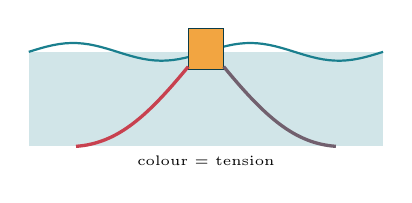
\begin{tikzpicture}[x=0.75cm,y=0.75cm]
      \fill[sea!20] (0,0) rectangle (6,1.6);
      \draw[sea, thick, domain=0:6, samples=60] plot (\x,{1.6+0.15*sin(deg(2*pi*\x/3))});
      \fill[sand, draw=deep] (2.7,1.3) rectangle (3.3,2.0);
      \draw[coral, very thick] (2.7,1.35) .. controls (2.0,0.5) and (1.5,0.05) .. (0.8,0);
      \draw[sea!50!coral, very thick] (3.3,1.35) .. controls (4.0,0.5) and (4.5,0.05) .. (5.2,0);
      \node[font=\tiny, below] at (3,0) {colour = tension};
    \end{tikzpicture}
  \end{columns}
\end{frame}

% ======================================================================
\sectionframe{Part 3}{HOS waves and validation}

% ----------------------------------------------------------------------
\begin{frame}[fragile]{\texttt{HOS\_FloatStepper/}: the moored box in HOS waves}
  \begin{columns}[T]
    \column{0.5\textwidth}
\begin{lstlisting}[language=foamb]
externalForcing   Grid2Grid;
Grid2GridCoeffs
{
    waveType                Grid2Grid;
    Grid2GridInputFileName  Grid2Grid.dict;
    referencePosition  (-9 0 0); // box: HOS x = 9
    referenceTheta     0;
    referenceTime      4;   // focused wave: 15
    Tsoft              0;
}
inletCoeffs           // externalSource, Tsoft 0
{ relaxationZone { startX (-2.5 0 -0.5);
                   endX   (-1.5 0  0.5); } }
outletCoeffs          // x = 1.5 .. 2.5
{ relaxationZone { ... } }
\end{lstlisting}
    \footnotesize\renewcommand{\arraystretch}{1.1}
    \begin{tabular}{@{}lrrr@{}}
      \toprule
      Case & CFD $t$=0 & end & medium \\
      \midrule
      \texttt{mooredBox} & HOS 4 s & 23 s & 24 min \\
      \texttt{...FocusedWave} & HOS 15 s & 15 s & 12 min \\
      \bottomrule
    \end{tabular}
    \column{0.47\textwidth}\small
    \begin{itemize}
      \item Same mesh, box, mooring and numerics as \texttt{FloatStepper/mooredBox}, solver
            \texttt{floatStepperWaveIsoFoam}
      \item 1 m relaxation zones at both ends, outside the morphing mesh
      \item Start in calm water at the box, as Day 2
      \item Wave: Day 1 \texttt{MooredBoxRegularWaves}, or a focused wave on the box at $t$ = 10 s
    \end{itemize}
\begin{lstlisting}[style=sh]
module load lapack/3.11.0 fftw/3.3.10  # DTU
./Allrun                # HOS, then CFD
MESH=coarse ./Allrun
python3 ../../../../Tools/compareHOS_CFD.py
\end{lstlisting}
    \scriptsize Regular-wave amplitudes ($t$ = 13--23 s): 92\,\% surge, 93\,\% heave, 89\,\% pitch of
    \texttt{FloatStepper/mooredBox}. The HOS piston adds a free second harmonic, so $H$ varies along the tank.
  \end{columns}
\end{frame}

% ----------------------------------------------------------------------
\begin{frame}{How good are the results?}
  \begin{columns}[T]
    \column{0.55\textwidth}\small
    Medium mesh, $t$ = 13--23 s, against the experiment (Wu et al., BOX3):

    \vspace{2mm}
    \renewcommand{\arraystretch}{1.3}
    \begin{tabularx}{\linewidth}{@{}P{2.2cm}L@{}}
      \toprule
      Quantity & Result \\
      \midrule
      Surge & {\leavevmode\color{sea}\bfseries good}: amplitude 8--11\,\% high \\
      Heave & {\leavevmode\color{sea}\bfseries good}: amplitude 4--6\,\% high \\
      Pitch & {\leavevmode\color{coral}\bfseries known model error}: about 80$^\circ$ late in phase, peak too high \\
      Line tension & {\leavevmode\color{sand!80!black}\bfseries fair}: amplitude 11--17\,\% low, the sharp peaks are missed \\
      \bottomrule
    \end{tabularx}
    \column{0.42\textwidth}\small
    \textbf{Caveats}
    \begin{itemize}
      \item The sign conventions of the experiment are inferred from the data (surge, pitch and load
            cell reversed), not documented
      \item Use surge and heave for validation
      \item The HOS wave has not been compared with the experiment
    \end{itemize}
    \textbf{For discussion}
    \begin{itemize}
      \item Why is pitch late? 2D slice vs.\ 3D lines, line damping, mesh, the mooring
            moment arm \dots
      \item Why are tension peaks missed? Snap loads, \texttt{dtM}, segment count, line
            elasticity
    \end{itemize}
  \end{columns}
\end{frame}

% ======================================================================
{\setbeamercolor{background canvas}{bg=deep}
 \setbeamertemplate{footline}{}
 \setbeamercolor{normal text}{fg=foam}
 \setbeamercolor{itemize/enumerate body}{fg=foam}
 \setbeamercolor{frametitle}{fg=white}
 \renewcommand{\key}[1]{{\leavevmode\ttfamily\color{sand}#1}}
 \renewcommand{\file}[1]{{\leavevmode\ttfamily\color{sand}#1}}
\begin{frame}[plain]{Hands-on: things to try}
  \small
  \begin{columns}[T]
    \column{0.48\textwidth}\color{foam}
    {\color{sand}\bfseries Mooring}
    \begin{itemize}
      \item Double \texttt{EA}, or shorten the lines by 5 cm: surge and tension?
      \item \texttt{NumSegs} 40 $\rightarrow$ 20: does the tension change?
      \item Remove the restraint: how far does the box drift in 23 s?
      \item Plot \texttt{FAIRTEN1} and \texttt{FAIRTEN3}: upstream vs.\ downstream line
      \item \texttt{mooringToParaview.py}: watch a line go slack
    \end{itemize}
    \column{0.48\textwidth}\color{foam}
    {\color{sand}\bfseries Body and flow}
    \begin{itemize}
      \item sixDoF vs.\ FloatStepper: same motion? same cost?
      \item \texttt{MESH=coarse} vs.\ medium: which motion is mesh-sensitive?
      \item \key{innerDistance}/\key{outerDistance}: cell quality at the largest pitch
      \item HOS focused wave: peak tension when the crest hits the box
      \item \texttt{waveStats.py}: is the wave at $x$ = $-1$ m the one you asked for?
    \end{itemize}
  \end{columns}
\end{frame}}

\end{document}
